\documentclass[
  shownotes,
  xcolor={svgnames},
  hyperref={colorlinks,citecolor=DarkBlue,linkcolor=andesred,urlcolor=DarkBlue}
  , aspectratio=169]{beamer}
\usepackage{animate}
\usepackage{amsmath}
\usepackage{amsfonts}
\usepackage{amssymb}
\usepackage{pifont}
\usepackage{mathpazo}
%\usepackage{xcolor}
\usepackage{multimedia}
\usepackage{fancybox}
\usepackage[para]{threeparttable}
\usepackage{multirow}
\setcounter{MaxMatrixCols}{30}
\usepackage{subcaption}
\usepackage{graphicx}
\usepackage{lscape}
\usepackage[compatibility=false,font=small]{caption}
\usepackage{booktabs}
\usepackage{ragged2e}
\usepackage{chronosys}
\usepackage{appendixnumberbeamer}
\usepackage{animate}
\setbeamertemplate{caption}[numbered]
\usepackage{color}
%\usepackage{times}
\usepackage{tikz}
\usepackage{comment} %to comment
%% BibTeX settings
\usepackage{natbib}
\bibliographystyle{apalike}
\bibpunct{(}{)}{,}{a}{,}{,}
\setbeamertemplate{bibliography item}{[\theenumiv]}

% Defines columns for bespoke tables
\usepackage{array}
\newcolumntype{L}[1]{>{\raggedright\let\newline\\\arraybackslash\hspace{0pt}}m{#1}}
\newcolumntype{C}[1]{>{\centering\let\newline\\\arraybackslash\hspace{0pt}}m{#1}}
\newcolumntype{R}[1]{>{\raggedleft\let\newline\\\arraybackslash\hspace{0pt}}m{#1}}


\usepackage{xfrac}


\usepackage{multicol}
\setlength{\columnsep}{0.5cm}

% Theme and colors
\usetheme{Boadilla}

% I define a custom pallete
\definecolor{andesred}{HTML}{1B175E}
\definecolor{andesyellow}{HTML}{ffff00}

% Other options
\providecommand{\U}[1]{\protect\rule{.1in}{.1in}}
\usefonttheme{serif}
\setbeamertemplate{itemize items}[default]
\setbeamertemplate{enumerate items}[square]
\setbeamertemplate{section in toc}[circle]


\definecolor{mybackground}{HTML}{1B175E}
\definecolor{myforeground}{HTML}{0000A0}

\setbeamercolor{normal text}{fg=black,bg=white}
\setbeamercolor{alerted text}{fg=andesred}
\setbeamercolor{example text}{fg=black}

\setbeamercolor{background canvas}{fg=myforeground, bg=white}
\setbeamercolor{background}{fg=myforeground, bg=mybackground}
\setbeamercolor{palette tertiary}{fg=myforeground,bg=mybackground}

\setbeamercolor{palette primary}{fg=black, bg=white}
\setbeamercolor{palette secondary}{fg=black, bg=white!10!andesyellow}
\setbeamercolor{palette tertiary}{fg=black, bg=white}


\setbeamercolor{frametitle}{fg=black}
\setbeamercolor{title}{fg=black}
\setbeamercolor{block title}{fg=andesred}
\setbeamercolor{itemize item}{fg=andesred}
\setbeamercolor{itemize subitem}{fg=andesred}
\setbeamercolor{itemize subsubitem}{fg=andesred}
\setbeamercolor{enumerate item}{fg=andesred}
\setbeamercolor{item projected}{bg=gray!30!white,fg=andesred}
\setbeamercolor{enumerate subitem}{fg=andesred}
\setbeamercolor{section number projected}{bg=gray!30!white,fg=andesred}
\setbeamercolor{section in toc}{fg=andesred}
\setbeamercolor{caption name}{fg=andesred}
\setbeamercolor{button}{bg=gray!30!white,fg=andesred}
\setbeamercolor{title in head/foot}{fg=andesred}



\usepackage{fancyvrb}
\newcommand{\VerbBar}{|}
\newcommand{\VERB}{\Verb[commandchars=\\\{\}]}
\DefineVerbatimEnvironment{Highlighting}{Verbatim}{commandchars=\\\{\}}
% Add ',fontsize=\small' for more characters per line
\usepackage{framed}
\definecolor{shadecolor}{RGB}{248,248,248}
\newenvironment{Shaded}{\begin{snugshade}}{\end{snugshade}}
\newcommand{\AlertTok}[1]{\textcolor[rgb]{0.94,0.16,0.16}{#1}}
\newcommand{\AnnotationTok}[1]{\textcolor[rgb]{0.56,0.35,0.01}{\textbf{\textit{#1}}}}
\newcommand{\AttributeTok}[1]{\textcolor[rgb]{0.77,0.63,0.00}{#1}}
\newcommand{\BaseNTok}[1]{\textcolor[rgb]{0.00,0.00,0.81}{#1}}
\newcommand{\BuiltInTok}[1]{#1}
\newcommand{\CharTok}[1]{\textcolor[rgb]{0.31,0.60,0.02}{#1}}
\newcommand{\CommentTok}[1]{\textcolor[rgb]{0.56,0.35,0.01}{\textit{#1}}}
\newcommand{\CommentVarTok}[1]{\textcolor[rgb]{0.56,0.35,0.01}{\textbf{\textit{#1}}}}
\newcommand{\ConstantTok}[1]{\textcolor[rgb]{0.00,0.00,0.00}{#1}}
\newcommand{\ControlFlowTok}[1]{\textcolor[rgb]{0.13,0.29,0.53}{\textbf{#1}}}
\newcommand{\DataTypeTok}[1]{\textcolor[rgb]{0.13,0.29,0.53}{#1}}
\newcommand{\DecValTok}[1]{\textcolor[rgb]{0.00,0.00,0.81}{#1}}
\newcommand{\DocumentationTok}[1]{\textcolor[rgb]{0.56,0.35,0.01}{\textbf{\textit{#1}}}}
\newcommand{\ErrorTok}[1]{\textcolor[rgb]{0.64,0.00,0.00}{\textbf{#1}}}
\newcommand{\ExtensionTok}[1]{#1}
\newcommand{\FloatTok}[1]{\textcolor[rgb]{0.00,0.00,0.81}{#1}}
\newcommand{\FunctionTok}[1]{\textcolor[rgb]{0.00,0.00,0.00}{#1}}
\newcommand{\ImportTok}[1]{#1}
\newcommand{\InformationTok}[1]{\textcolor[rgb]{0.56,0.35,0.01}{\textbf{\textit{#1}}}}
\newcommand{\KeywordTok}[1]{\textcolor[rgb]{0.13,0.29,0.53}{\textbf{#1}}}
\newcommand{\NormalTok}[1]{#1}
\newcommand{\OperatorTok}[1]{\textcolor[rgb]{0.81,0.36,0.00}{\textbf{#1}}}
\newcommand{\OtherTok}[1]{\textcolor[rgb]{0.56,0.35,0.01}{#1}}
\newcommand{\PreprocessorTok}[1]{\textcolor[rgb]{0.56,0.35,0.01}{\textit{#1}}}
\newcommand{\RegionMarkerTok}[1]{#1}
\newcommand{\SpecialCharTok}[1]{\textcolor[rgb]{0.00,0.00,0.00}{#1}}
\newcommand{\SpecialStringTok}[1]{\textcolor[rgb]{0.31,0.60,0.02}{#1}}
\newcommand{\StringTok}[1]{\textcolor[rgb]{0.31,0.60,0.02}{#1}}
\newcommand{\VariableTok}[1]{\textcolor[rgb]{0.00,0.00,0.00}{#1}}
\newcommand{\VerbatimStringTok}[1]{\textcolor[rgb]{0.31,0.60,0.02}{#1}}
\newcommand{\WarningTok}[1]{\textcolor[rgb]{0.56,0.35,0.01}{\textbf{\textit{#1}}}}
\usepackage{graphicx}
\makeatletter

\makeatother






%%%%%%%%%%%%%%% BEGINS DOCUMENT %%%%%%%%%%%%%%%%%%

\AtBeginSection[]
{
    \begin{frame}
        \frametitle{Agenda}
        \tableofcontents[currentsection]
    \end{frame}
}

\begin{document}

\title{The Predictive Paradigm}
\subtitle{Big Data y Machine Learning para Economía Aplicada}
\date{}

\author[Sarmiento-Barbieri]{Ignacio Sarmiento-Barbieri}
\institute[Uniandes]{Universidad de los Andes}


\begin{frame}[noframenumbering]
\maketitle
\end{frame}

%%%%%%%%%%%%%%%%%%%%%%%%%%%%%%%%%%%
%       Motivation              %
% What is the question?
% Why do we care?
% What is new?
% What do you find?
%%%%%%%%%%%%%%%%%%%%%%%%%%%%%%%%%%%




\begin{frame}
\frametitle{Agenda}

\tableofcontents


\end{frame}

%----------------------------------------------------------------------%
%----------------------------------------------------------------------%
\section{About the Course}
%----------------------------------------------------------------------%
%----------------------------------------------------------------------%

%----------------------------------------------------------------------%

%----------------------------------------------------------------------%
\begin{frame}
\frametitle{¿Qué entendemos por Big Data y ML?}

\begin{itemize}
      \item ¿Que es Big Data? 
      \medskip
      \begin{itemize}

      \item Big n, es solo parte de la historia
      \medskip
      \item Big también es big k, muchos covariates, a veces $n<<k$
      \medskip
      \item Vamos a entender Big también como datos que no surgen de fuentes tradicionales (cuentas nac., GEIH, etc)
      \medskip
      \begin{itemize}
        \item Datos de la Web, Geográficos, etc.

      \end{itemize}
      \end{itemize}
      \medskip
      \item Machine Learning
      \medskip
        \begin{itemize}

          \item Cambio de paradigma de estimación a predicción

        \end{itemize} 
      
\end{itemize}

\end{frame}
%----------------------------------------------------------------------%
\begin{frame}
\frametitle{Lenguajes}


\begin{minipage}[t]{0.58\linewidth}
        \begin{itemize}
            \item Estadística y Econometría
           \medskip
            \item Inglés
           \medskip
            \item Código
            %Uno de los objetivos implícitos es que mejoren sus habilidades para escribir código y usar herramientas de la industria
            \begin{itemize}
              \item Elijan el que quieran: 
              \begin{itemize}
                \item \texttt{R}, \texttt{Python}, o cualquier otro
                \item no hay restricción
                \item yo me basare en \texttt{R}
                \end{itemize}
              \item Github
              \item Slack
              
            \end{itemize}
            \item Aprender haciendo y mucha prueba y error! 
            
        \end{itemize}
    \end{minipage}
    \hfill
    \begin{minipage}[t]{0.38\linewidth}%
        \begin{figure}[H] \centering
            \captionsetup{justification=centering}  
            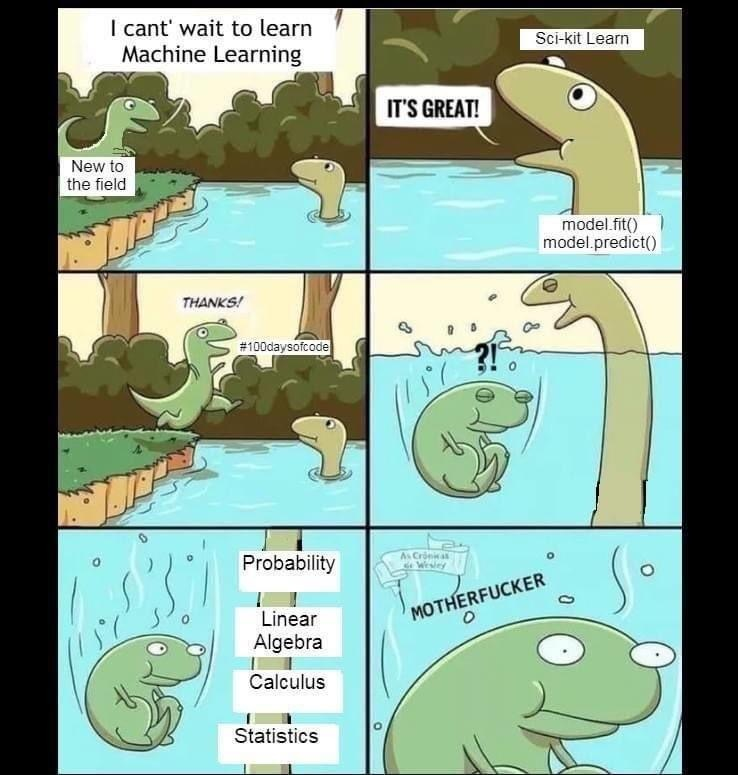
\includegraphics[scale=0.2]{figures/ml_trick}
    \end{figure}
    \end{minipage}

\end{frame}


%----------------------------------------------------------------------%

\begin{frame}
\frametitle{Materiales}


\begin{enumerate}
  \item Bloque Neón
  \medskip
  \item Statistical Learning (FREE!!! (as beer, not speech)) \url{https://www.gnu.org/philosophy/free-sw.en.html}
  \medskip
  \begin{itemize}
    \small
    \item James, G., Witten, D., Hastie, T., \& Tibshirani, R. (2013). An introduction to statistical learning (ISLR)
    \medskip
    \item Hastie, T., Tibshirani, R., \& Friedman, J. (2009). The elements of statistical learning: data mining, inference, and prediction
  \end{itemize}
  \medskip
  \item Libros de econometría
  \begin{itemize}
    \small
    \item Davidson, R., \& MacKinnon, J. G. (2004). Econometric theory and methods 
    \medskip
    \item Wooldridge, J. M. (2010). Econometric analysis of cross section and panel data. 
    \medskip
    \item Hayashi, F. (2000). Econometrics
  \end{itemize}
\bigskip
  \end{enumerate}



%  \begin{itemize}
%    \item La idea es movernos hacia adelante y al costado de la econometria de grado
%    \item Armar un puente entre los Economistas y los Machine Learners, Computer Scientists
%    \item Pensar el curso como un ISLR/Elements pero para economistas
%\end{itemize}


\end{frame}

%----------------------------------------------------------------------%
%----------------------------------------------------------------------%
\section{Machine learning is all about prediction}
%----------------------------------------------------------------------%
%----------------------------------------------------------------------%

%----------------------------------------------------------------------%
\begin{frame}
\frametitle{Machine learning is all about prediction}

\begin{itemize}
  \item Machine learning is a branch of computer science and statistics, tasked with developing algorithms to predict outcomes $y$ from observable variables $x$.
  \medskip
  \item The learning part comes from the fact that we don't specify how exactly the computer should predict $y$  from $x$. This is left as an empirical problem that the computer can “learn”.
\medskip
  \item In general, this means that we abstract from the underlying model, the approach is  pragmatic

  
  \bigskip
  \bigskip

  \pause
  \begin{quote}
  \centering
  \bf ``Whatever works, works....''
  \end{quote}
\end{itemize}
\end{frame}
%----------------------------------------------------------------------%
\begin{frame}
\frametitle{``Whatever works, works....''}



\begin{figure}[H] \centering
            \captionsetup{justification=centering}  
            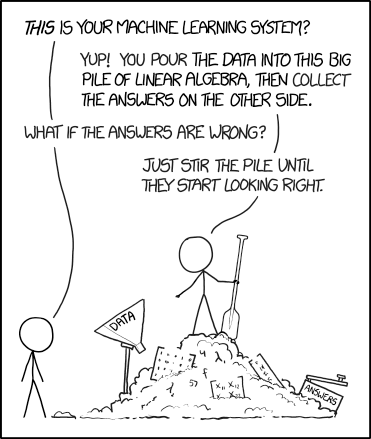
\includegraphics[scale=0.45]{figures/machine_learning}
\end{figure}


\end{frame}
%----------------------------------------------------------------------%
\begin{frame}
\frametitle{``Whatever works, works....''????}


\begin{itemize}
\item In many applications, ML techniques can be successfully applied by data scientists with little knowledge of the problem domain. 

\medskip
\item For example, the company Kaggle hosts prediction competitions (\url{www.kaggle.com/competitions}) in which a sponsor provides a data set, and contestants around the world can submit entries, often predicting successfully despite limited context about the problem.

\end{itemize}

\end{frame}
%----------------------------------------------------------------------%
\begin{frame}
\frametitle{``Whatever works, works....''????}


\begin{itemize}

  \item  However, much less attention has been paid to the limitations of pure prediction methods. 
\medskip
  \item When ML applications are used ``off the shelf'' without understanding the underlying assumptions or ensuring that conditions like stability are met, then the validity and usefulness of the conclusions can be compromised. 

  \medskip
  \item A deeper question concerns whether a given problem can be solved using only techniques for prediction, or whether statistical approaches to estimating the causal effect of an intervention are required.

\end{itemize}

\end{frame}
%----------------------------------------------------------------------%
%----------------------------------------------------------------------%
\section{Prediction vs Causality}
%----------------------------------------------------------------------%
%----------------------------------------------------------------------%

\begin{frame}
\frametitle{Policy Prediction Problems}

\begin{itemize}


\item Empirical policy research often focuses on causal inference. 
\medskip
\item Since policy choices seem to depend on understanding the counterfactual— what happens with and without a policy—this tight link of causality and policy seems natural. 
\medskip
\item  While this link holds in many cases, there are also many policy applications where causal inference is not central, or even necessary.
\end{itemize}

\end{frame}




%----------------------------------------------------------------------%
\begin{frame}
\frametitle{The Causal Paradigm}


\begin{align}
y=f(X)+u
\end{align}
\medskip
\begin{itemize}
  \item Interest lies on inference
  \medskip
  \item "Correct" $f()$ to understand how $y$ is affected by $X$
  \medskip
  \item Model: Theory, experiment
  \medskip
  \item Hypothesis testing (std. err., tests)
\end{itemize}

\end{frame}


%----------------------------------------------------------------------%

\begin{frame}
\frametitle{The Predictive Paradigm}


\begin{align}
y=f(X)+u
\end{align}

\begin{itemize}
  \item Interest on predicting $y$
  \medskip
  \item "Correct" $f()$ to be able to predict (no inference!)
  \medskip
  \item Model? We  treat $f()$ as a black box, and any approximation $\hat{f}()$ that yields a good prediction is good enough ({\it Whatever works, works.}).

\end{itemize}


\end{frame}
%----------------------------------------------------------------------%
\begin{frame}
\frametitle{Prediction vs. Causality}



\begin{minipage}[t]{0.45\linewidth}
        \begin{figure}[H] \centering
            \captionsetup{justification=centering}  
            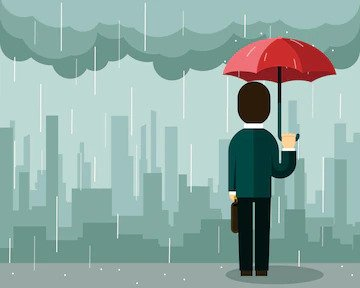
\includegraphics[scale=0.3]{figures/umbrella.jpg}
            \caption*{\bf Prepare}
    \end{figure}
    \end{minipage}
    \hfill
    \begin{minipage}[t]{0.45\linewidth}%
        \begin{figure}[H] \centering
            \captionsetup{justification=centering}  
            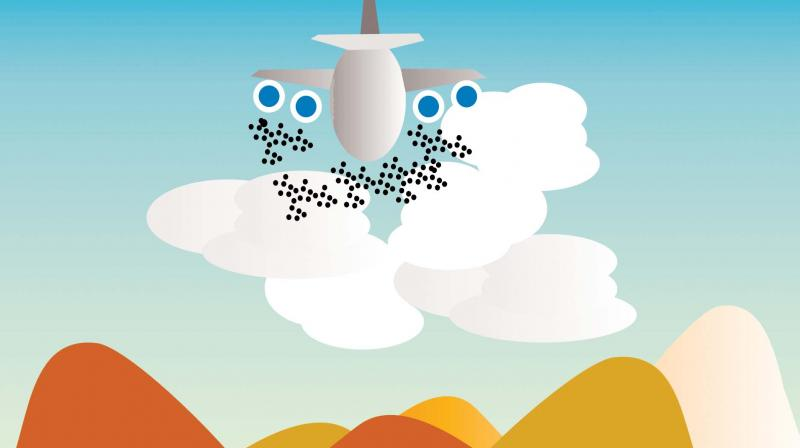
\includegraphics[scale=0.2]{figures/seeding.jpeg}
            \caption*{\bf Influence}
    \end{figure}
    \end{minipage}

\end{frame}
%----------------------------------------------------------------------%
\begin{frame}
\frametitle{Prediction vs. Causality}



\begin{minipage}[t]{0.45\linewidth}
       \begin{center}
        {\bf Prepare}
       \end{center}
       

       \begin{itemize}
       \item A loan officer wants to know the likelihood of an individual repaying a loan based on income, employment, and other characteristics.
       \end{itemize}
    \end{minipage}
    \hfill
    \begin{minipage}[t]{0.45\linewidth}%
    \begin{center}
        {\bf Influence}
       \end{center}
        

       \begin{itemize}
       \item A mortgage lender wants to know if direct debit will increase loan repayments.
       \end{itemize}
    
    \end{minipage}



\end{frame}
%----------------------------------------------------------------------%
\begin{frame}
\frametitle{Prediction vs. Causality}



\begin{minipage}[t]{0.45\linewidth}
       \begin{center}
        {\bf Prepare}
       \end{center}
       

       \begin{itemize}
       \item In order to decide whether to invest in a start-up, an investor needs to know how likely the start-up is to succeed, given the entrepreneur's experience and the characteristics of the industry.
       \end{itemize}
    \end{minipage}
    \hfill
    \begin{minipage}[t]{0.45\linewidth}%
    \begin{center}
        {\bf Influence}
       \end{center}
        

       \begin{itemize}
       \item An entrepreneur needs to know what the effect of receiving funding from a private equity investor (rather than getting a loan) is on the ultimate success of an enterprise.
       \end{itemize}
    
    \end{minipage}



\end{frame}
%----------------------------------------------------------------------%
\begin{frame}
\frametitle{Prediction vs. Causality}



\begin{minipage}[t]{0.45\linewidth}
       \begin{center}
        {\bf Prepare}
       \end{center}
       

       \begin{itemize}
       \item A home seller wants to know what price homes with the characteristics of his or her home typically sell for.
       \end{itemize}
    \end{minipage}
    \hfill
    \begin{minipage}[t]{0.45\linewidth}%
    \begin{center}
        {\bf Influence}
       \end{center}
        

       \begin{itemize}
       \item A home seller wants to know by how much installing new windows will raise the value of his or her home.
       \end{itemize}
    
    \end{minipage}

\end{frame}


%----------------------------------------------------------------------%
\begin{frame}
\frametitle{Prediction vs. Causality: Target}

\begin{align}
y&= f(x) +\epsilon \\
y&= \alpha + \beta x +\epsilon 
\end{align}
  \begin{figure}[H] \centering
            \captionsetup{justification=centering}  
            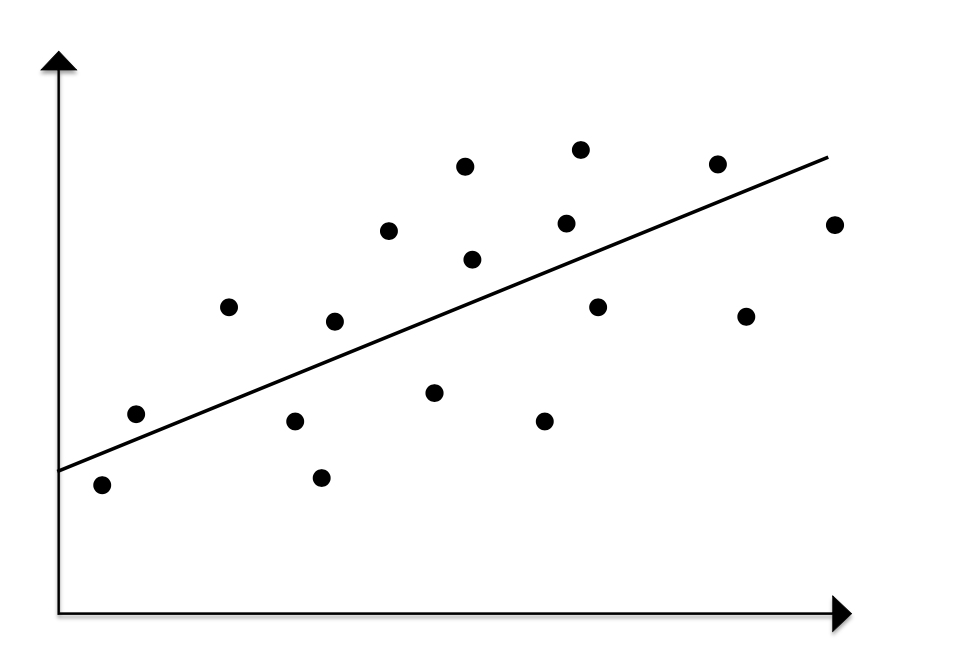
\includegraphics[scale=0.4]{figures/target1.png}
            
    \end{figure}

\end{frame}


%----------------------------------------------------------------------%
\begin{frame}
\frametitle{Prediction vs. Causality: Target}

\begin{align}
y= \underset{\textcolor{blue}{\hat{y}}}{\underbrace{\alpha+\beta x}}+\epsilon
\end{align}
  \begin{figure}[H] \centering
            \captionsetup{justification=centering}  
            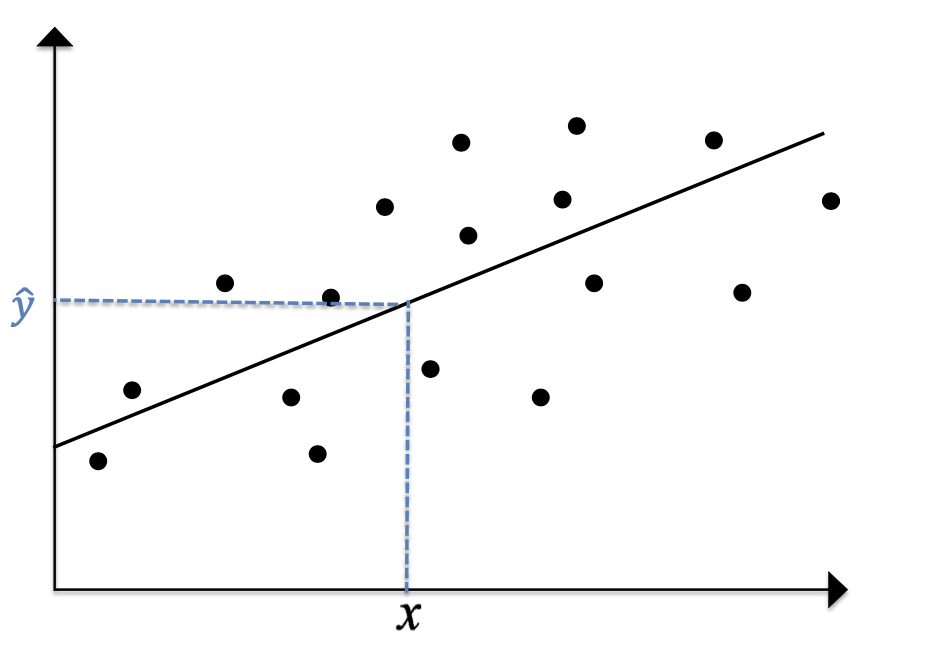
\includegraphics[scale=0.4]{figures/target2.png}
            
    \end{figure}

\end{frame}
%----------------------------------------------------------------------%
\begin{frame}
\frametitle{Prediction vs. Causality: Target}

\begin{align}
y= \alpha+\textcolor{blue}{\beta} x+\epsilon
\end{align}
  \begin{figure}[H] \centering
            \captionsetup{justification=centering}  
            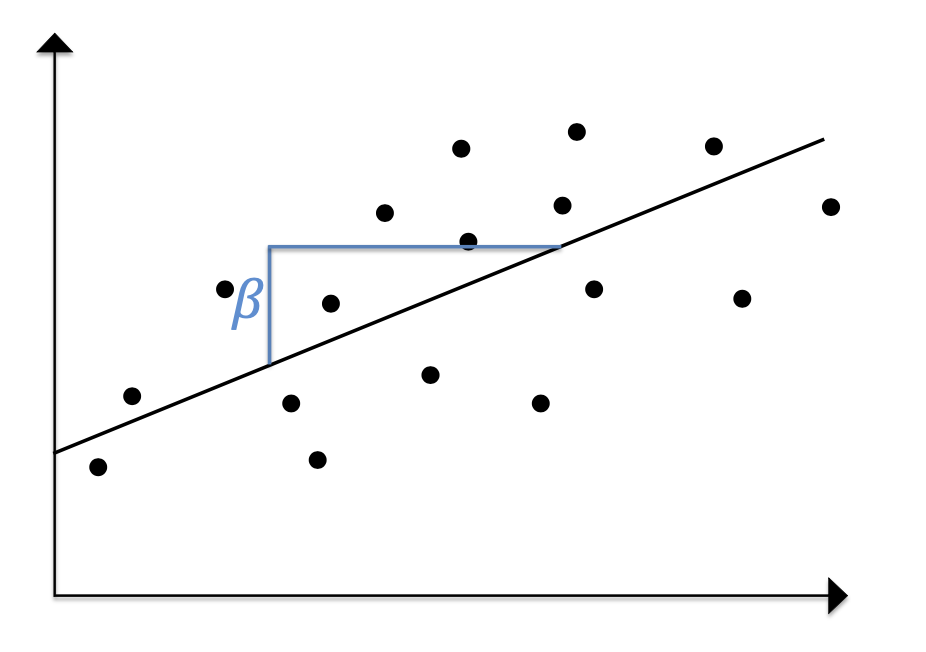
\includegraphics[scale=0.4]{figures/target3.png}
            
    \end{figure}

\end{frame}

%----------------------------------------------------------------------%
\begin{frame}
\frametitle{Prediction vs. Causality: The garden of the parallel paths?}

\begin{itemize}

\item We've seen that prediction and causality 
\medskip
  \begin{itemize}
    \item Answer different questions
    \medskip
    \item Serve different purposes
    \medskip
    \item Seek different targets
    \medskip
  \end{itemize}
\item Different strokes for different folks, or complementary tools in an applied economist's toolkit?
\end{itemize}

\end{frame}
%----------------------------------------------------------------------%
%----------------------------------------------------------------------%
\section{Prediction and loss functions}
%----------------------------------------------------------------------%
%----------------------------------------------------------------------%
%----------------------------------------------------------------------%
\begin{frame}
\frametitle{Getting serious about prediction}


\begin{align}
y=f(X)+u
\end{align}

\begin{itemize}
  \item Interest on predicting $Y$
  \medskip
  \item Model? We  treat $f()$ as a black box, and any approximation $\hat{f}()$ that yields a good prediction is good enough ({\it ``Whatever works, works...''}).
  \medskip
  \item How do we measure ``what works''?
  \pause
  \medskip
  \item Formal statistics can help  figure out this: what is a good prediction.

\end{itemize}

\end{frame}
%----------------------------------------------------------------------%
\begin{frame}
\frametitle{Minimizing our losses}

\begin{itemize}
\item Want our prediction to be ``close'' i.e. minimize the expected loss function
\medskip
\item Formally, a supervised learning algorithm takes as an input a loss function  $L(\hat{y},y)$
\medskip

and searches for a function $\hat{f}$ within a function class ${\mathcal{F}}$ that has a low expected prediction loss 
\begin{align}
E_{(y,X)}[L(\hat{f}(X),y)] 
\end{align}

on a new data point from the same distribution.

  \begin{figure}[H] \centering
            \captionsetup{justification=centering}  
            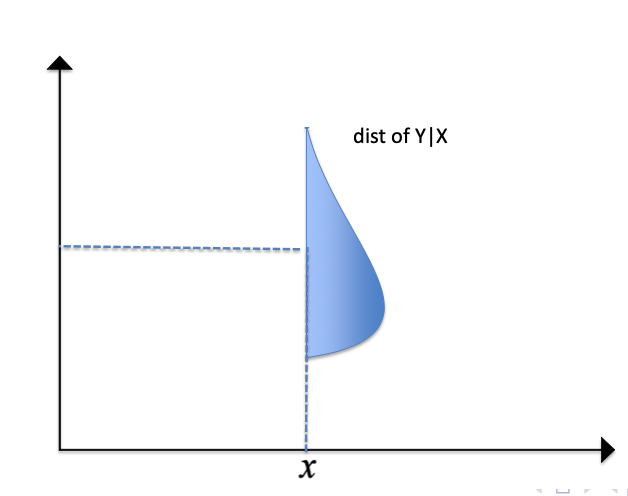
\includegraphics[scale=0.4]{figures/cond_distrib1.png}
            
    \end{figure}

\end{itemize}


\end{frame}
%----------------------------------------------------------------------%
\begin{frame}
\frametitle{Minimizing our losses}


\begin{itemize}
\item A very common loss function in a regression setting is the squared loss $L(d)=d^2$
\medskip
\item Under this loss function the expected prediction loss  is the mean squared error (MSE)
\medskip
\item Can we find the function $f^*$ within a function class ${\mathcal{F}}$ that has a low expected prediction loss?

\end{itemize}


\end{frame}
%----------------------------------------------------------------------%
\begin{frame}
\frametitle{Minimizing our losses}
\begin{itemize}

  
  \item By conditioning on X, it suffices to minimize  the $MSE(f)$ point wise so
  \medskip


\begin{align}
  f(x)= argmin_{f^*} E_{Y|X} [(Y-f^*)^2|X=x)
\end{align}



\item $f^*$ a random variable and we can treat $f^*$ as a constant (predictor)


\begin{align}
min_m E(Y-f^*)^2= \int (y-f^*)^2  f(y)dy
\end{align}

\item {\bf Result}: The best prediction of $Y$ at any point $X = x$ is the conditional mean, when best is measured using a square error loss
\end{itemize}

\end{frame}
%----------------------------------------------------------------------%
\begin{frame}
\frametitle{Minimizing our losses}
\begin{itemize}
\item {\bf Result}: The best prediction of $y$ at any point $X = x$ is the conditional mean, when best is measured using a square error loss
\end{itemize}
\begin{align}
f^* = E[y|X=x]
\end{align}

  \begin{figure}[H] \centering
            \captionsetup{justification=centering}  
            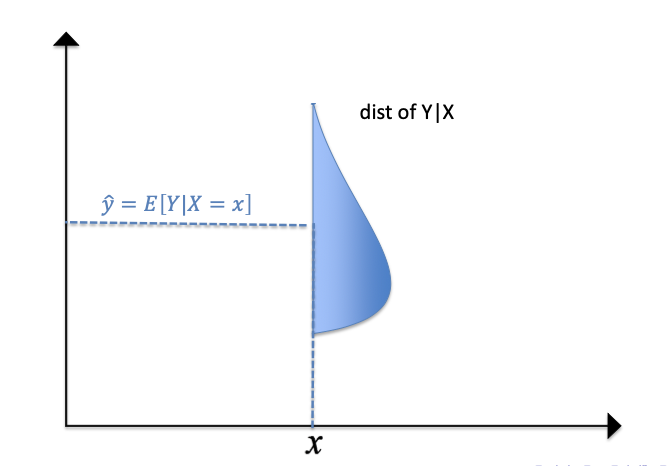
\includegraphics[scale=0.6]{figures/cond_distrib2.png}
            
    \end{figure}

\end{frame}
%----------------------------------------------------------------------%
\begin{frame}
\frametitle{Minimizing our losses}

\begin{itemize}
\item Prediction problem solved if we knew $f^* = E[y|X=x]$ 
\pause
\medskip
\item But we have to settle for an estimate: $\hat{f}(x)$
\medskip
\item The EMSE of this

\begin{align}
E(y-\hat y)^2 &= E(f(X)+u - \hat f(X))^2 
\end{align}
\end{itemize}

\end{frame}




%----------------------------------------------------------------------%
\begin{frame}[fragile]
\frametitle{Review}
  

\begin{itemize}
 \item The predictive paradigm 
 \medskip
    \begin{itemize} 
        \item Machine Learning is all about prediction
         \medskip
         \item ML targets something different than causal inference, they can complement each other
         \medskip
         
      \end{itemize}
  \item Next Class: Bias/Variance Trade Off and Linear Regression

    \end{itemize}

\end{frame}



%----------------------------------------------------------------------%
\end{document}
